


\section{Auswertung}
\label{sec:auswertung}

In diesem Kapitel werden die aufgenommenen Messwerte ausgewertet.
\subsection{Der Invertierende-Linearverstärker}
\label{sec:linearverstaerker}
\begin{figure}
    \centering
    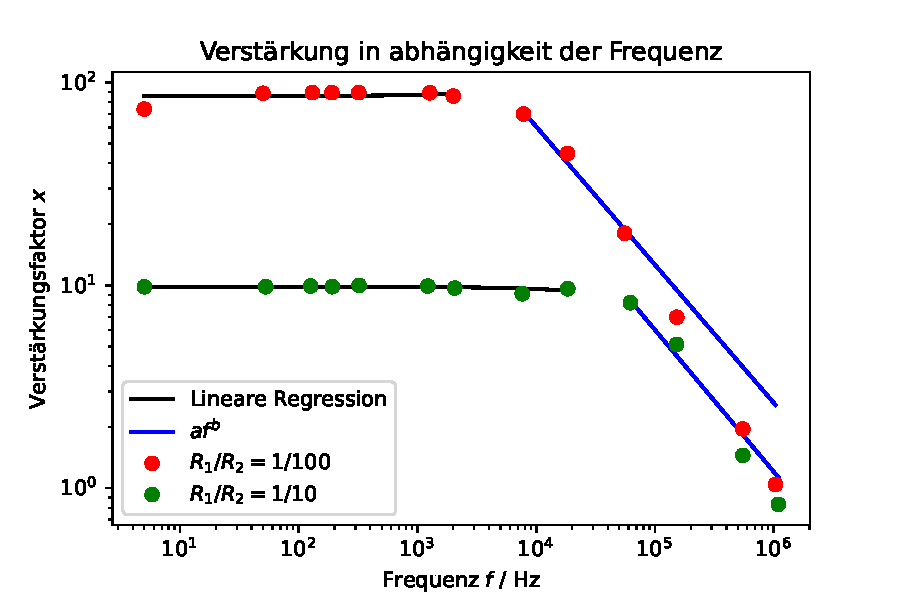
\includegraphics{content/grafiken/verstaerkung.pdf}
    \caption{Verstärkungskurve des als invertierenden Linearverstärker geschalteten Operationsverstärkers nach Eingangsfrequenz.}
    \label{fig:linearverstaerker}
  \end{figure}

  \begin{figure}
    \centering
    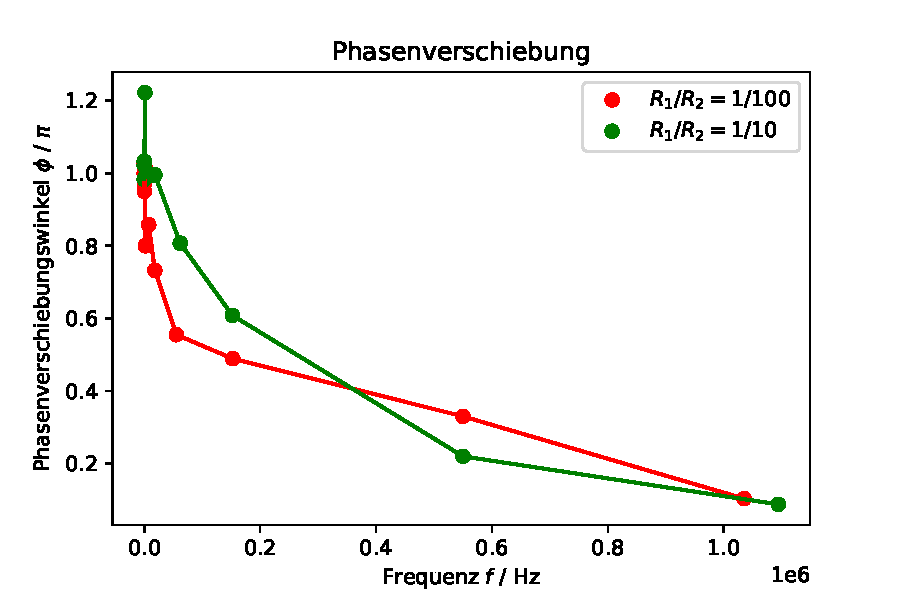
\includegraphics{content/grafiken/phasenverschiebung.pdf}
    \caption{Phasenverschiebung am invertierenden Linearverstärker in Abhängigkeit der Zugangsfrequenz.}
    \label{fig:phasenverschiebung}
  \end{figure}



\subsection{Der Umkehrintegrator und der invertierender Differenzierer}
\label{sec:umkehrintegrator}
\begin{figure}
    \centering
    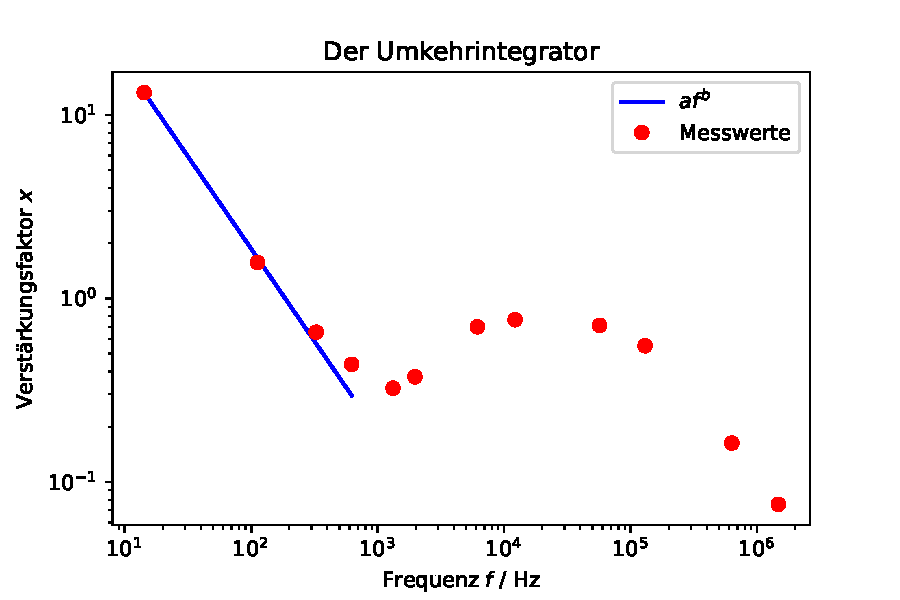
\includegraphics{content/grafiken/umkehrintegrator.pdf}
    \caption{Verstärkungskurve des Umkehrintegrators nach Eingangsfrequenz}
    \label{fig:umkehrintegrator}
  \end{figure}


  \begin{figure}
    \centering
    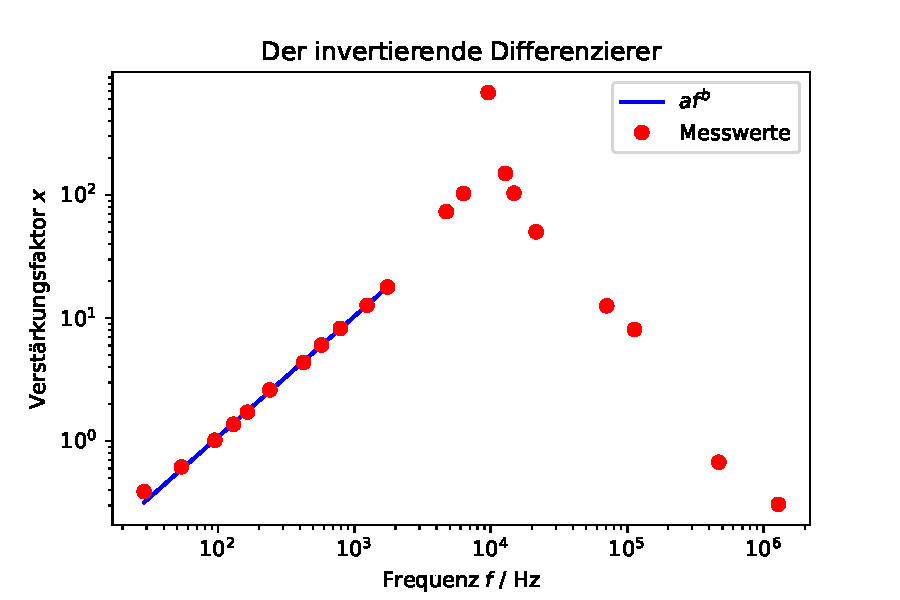
\includegraphics{content/grafiken/invdifferenzierer.pdf}
    \caption{Verstärkungskurve des invertierenden Differenzierers nach Eingangsfrequenz.}
    \label{fig:invdifferenzierer}
  \end{figure}





\subsection{Nicht-invertierender-Schmitt-Trigger}
\label{sec:schmitt}
\begin{figure}
    \centering
    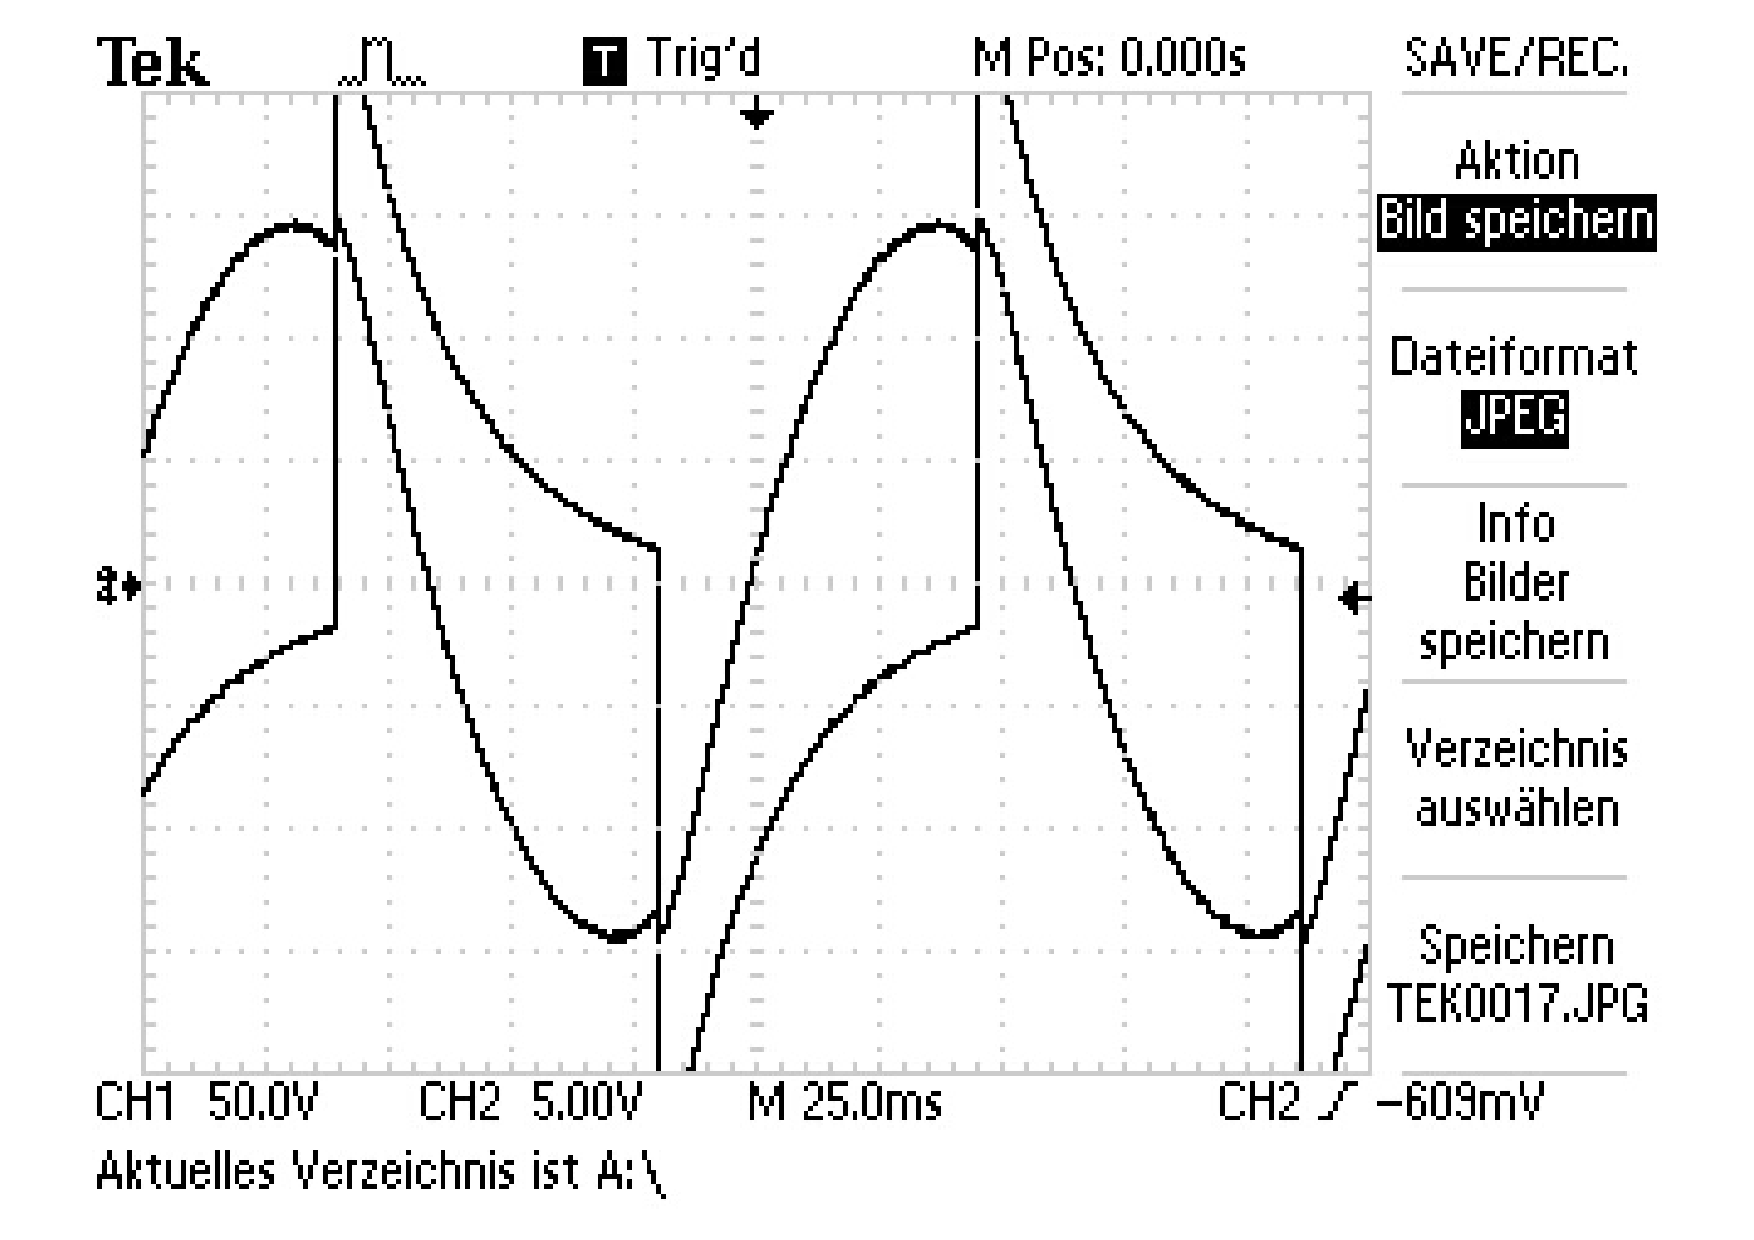
\includegraphics[width=1\textwidth]{content/grafiken/schmittTrigger/TEK0017.pdf}
    \caption{Oszilloskopbild des Spannungsverlaufs am invertierenden Schmitttrigger.}
    \label{fig:schmitttrigger}
  \end{figure}




























